\documentclass[14pt]{extbook}
\usepackage{multicol, enumerate, enumitem, hyperref, color, soul, setspace, parskip, fancyhdr} %General Packages
\usepackage{amssymb, amsthm, amsmath, latexsym, units, mathtools} %Math Packages
\everymath{\displaystyle} %All math in Display Style
% Packages with additional options
\usepackage[headsep=0.5cm,headheight=12pt, left=1 in,right= 1 in,top= 1 in,bottom= 1 in]{geometry}
\usepackage[usenames,dvipsnames]{xcolor}
\usepackage{dashrule}  % Package to use the command below to create lines between items
\newcommand{\litem}[1]{\item#1\hspace*{-1cm}\rule{\textwidth}{0.4pt}}
\pagestyle{fancy}
\lhead{Progress Quiz 7}
\chead{}
\rhead{Version ALL}
\lfoot{3510-5252}
\cfoot{}
\rfoot{Summer C 2021}
\begin{document}

\begin{enumerate}
\litem{
Write the equation of the graph presented below in the form $f(x)=ax^2+bx+c$, assuming  $a=1$ or $a=-1$. Then, choose the intervals that $a, b,$ and $c$ belong to.
\begin{center}
    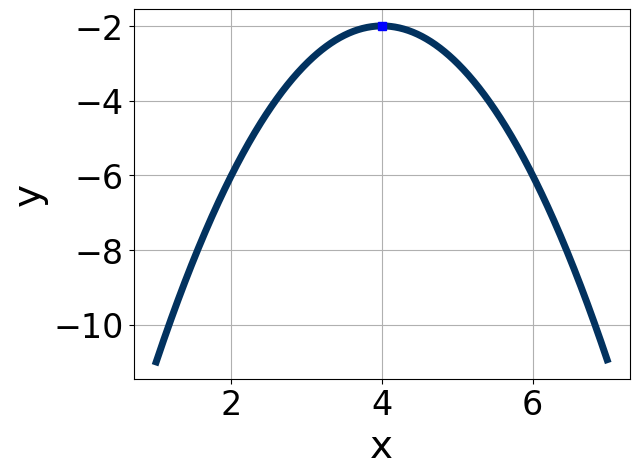
\includegraphics[width=0.5\textwidth]{../Figures/quadraticGraphToEquationA.png}
\end{center}
\begin{enumerate}[label=\Alph*.]
\item \( a \in [-1.3, 0], \hspace*{5mm} b \in [4, 10], \text{ and } \hspace*{5mm} c \in [-18, -16] \)
\item \( a \in [0.4, 1.5], \hspace*{5mm} b \in [4, 10], \text{ and } \hspace*{5mm} c \in [10, 15] \)
\item \( a \in [0.4, 1.5], \hspace*{5mm} b \in [-10, -5], \text{ and } \hspace*{5mm} c \in [10, 15] \)
\item \( a \in [-1.3, 0], \hspace*{5mm} b \in [-10, -5], \text{ and } \hspace*{5mm} c \in [-18, -16] \)
\item \( a \in [-1.3, 0], \hspace*{5mm} b \in [-10, -5], \text{ and } \hspace*{5mm} c \in [-14, -9] \)

\end{enumerate} }
\litem{
Solve the quadratic equation below. Then, choose the intervals that the solutions $x_1$ and $x_2$ belong to, with $x_1 \leq x_2$.\[ 25x^{2} -60 x + 36 = 0 \]\begin{enumerate}[label=\Alph*.]
\item \( x_1 \in [-0.17, 0.3] \text{ and } x_2 \in [5.29, 6.08] \)
\item \( x_1 \in [0.41, 0.76] \text{ and } x_2 \in [2.12, 2.75] \)
\item \( x_1 \in [0.34, 0.44] \text{ and } x_2 \in [2.63, 4.78] \)
\item \( x_1 \in [1.11, 1.3] \text{ and } x_2 \in [0.47, 1.4] \)
\item \( x_1 \in [29.67, 30.12] \text{ and } x_2 \in [29.21, 30.44] \)

\end{enumerate} }
\litem{
Factor the quadratic below. Then, choose the intervals that contain the constants in the form $(ax+b)(cx+d); b \leq d.$\[ 24x^{2} +2 x -15 \]\begin{enumerate}[label=\Alph*.]
\item \( a \in [10.31, 12.79], \hspace*{5mm} b \in [-3, 0], \hspace*{5mm} c \in [1.45, 3.07], \text{ and } \hspace*{5mm} d \in [0, 7] \)
\item \( a \in [1.21, 2.53], \hspace*{5mm} b \in [-3, 0], \hspace*{5mm} c \in [11.98, 12.04], \text{ and } \hspace*{5mm} d \in [0, 7] \)
\item \( a \in [0.14, 1.79], \hspace*{5mm} b \in [-20, -12], \hspace*{5mm} c \in [-0.18, 1.72], \text{ and } \hspace*{5mm} d \in [18, 22] \)
\item \( a \in [2.38, 4.11], \hspace*{5mm} b \in [-3, 0], \hspace*{5mm} c \in [4.37, 6.28], \text{ and } \hspace*{5mm} d \in [0, 7] \)
\item \( \text{None of the above.} \)

\end{enumerate} }
\litem{
Write the equation of the graph presented below in the form $f(x)=ax^2+bx+c$, assuming  $a=1$ or $a=-1$. Then, choose the intervals that $a, b,$ and $c$ belong to.
\begin{center}
    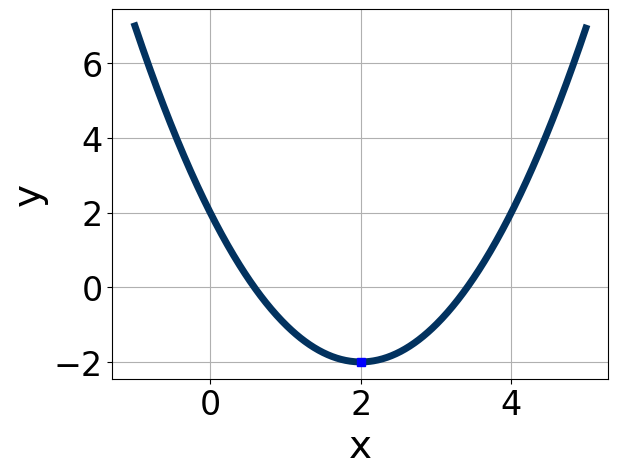
\includegraphics[width=0.5\textwidth]{../Figures/quadraticGraphToEquationCopyA.png}
\end{center}
\begin{enumerate}[label=\Alph*.]
\item \( a \in [1, 3], \hspace*{5mm} b \in [-6, -3], \text{ and } \hspace*{5mm} c \in [1, 4] \)
\item \( a \in [-2, 0], \hspace*{5mm} b \in [-6, -3], \text{ and } \hspace*{5mm} c \in [-7, -4] \)
\item \( a \in [-2, 0], \hspace*{5mm} b \in [3, 7], \text{ and } \hspace*{5mm} c \in [-7, -4] \)
\item \( a \in [1, 3], \hspace*{5mm} b \in [3, 7], \text{ and } \hspace*{5mm} c \in [1, 4] \)
\item \( a \in [1, 3], \hspace*{5mm} b \in [3, 7], \text{ and } \hspace*{5mm} c \in [6, 8] \)

\end{enumerate} }
\litem{
Graph the equation below.\[ f(x) = (x-1)^2 - 15 \]\begin{enumerate}[label=\Alph*.]
\begin{multicols}{2}\item 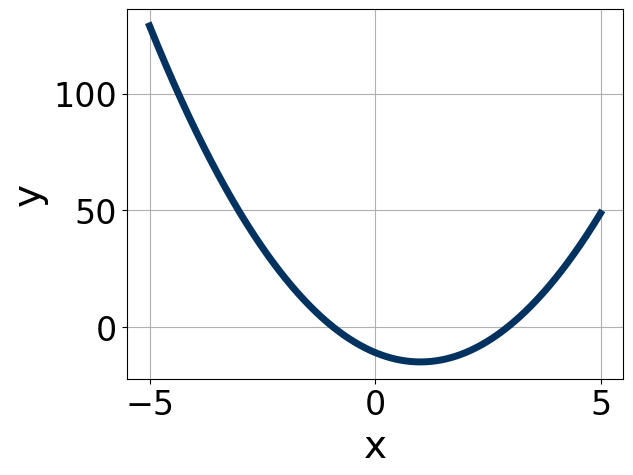
\includegraphics[width = 0.3\textwidth]{../Figures/quadraticEquationToGraphAA.png}\item 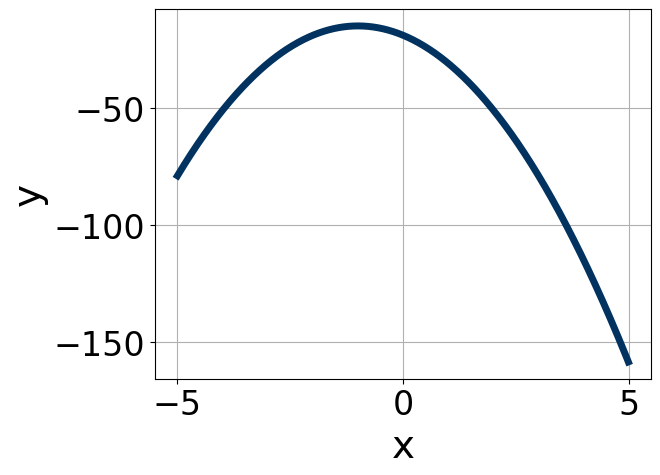
\includegraphics[width = 0.3\textwidth]{../Figures/quadraticEquationToGraphBA.png}\item 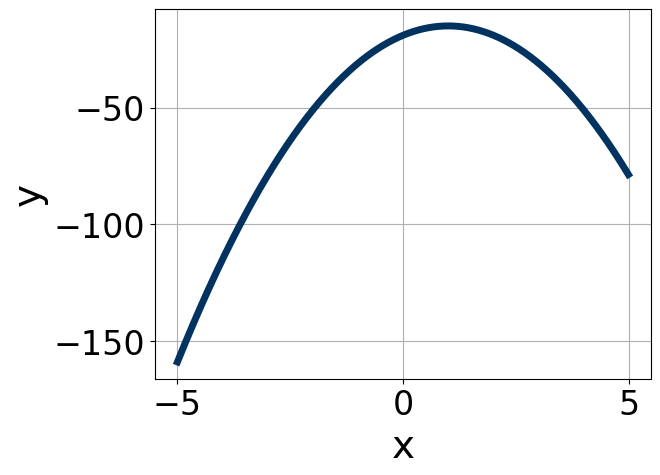
\includegraphics[width = 0.3\textwidth]{../Figures/quadraticEquationToGraphCA.png}\item 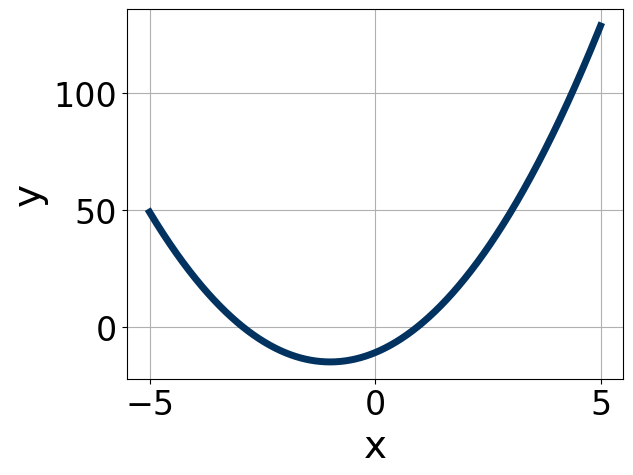
\includegraphics[width = 0.3\textwidth]{../Figures/quadraticEquationToGraphDA.png}\end{multicols}\item None of the above.
\end{enumerate} }
\litem{
Solve the quadratic equation below. Then, choose the intervals that the solutions belong to, with $x_1 \leq x_2$ (if they exist).\[ -19x^{2} -13 x + 4 = 0 \]\begin{enumerate}[label=\Alph*.]
\item \( x_1 \in [-2.01, -0.76] \text{ and } x_2 \in [-0.3, 0.68] \)
\item \( x_1 \in [-23.26, -21.68] \text{ and } x_2 \in [21.39, 22.14] \)
\item \( x_1 \in [-0.7, 0.91] \text{ and } x_2 \in [0.37, 1.52] \)
\item \( x_1 \in [-5.5, -3.85] \text{ and } x_2 \in [17.2, 17.52] \)
\item \( \text{There are no Real solutions.} \)

\end{enumerate} }
\litem{
Solve the quadratic equation below. Then, choose the intervals that the solutions $x_1$ and $x_2$ belong to, with $x_1 \leq x_2$.\[ 12x^{2} -11 x -36 = 0 \]\begin{enumerate}[label=\Alph*.]
\item \( x_1 \in [-16.44, -15.72] \text{ and } x_2 \in [26.49, 27.56] \)
\item \( x_1 \in [-3.53, -2.27] \text{ and } x_2 \in [1.11, 1.35] \)
\item \( x_1 \in [-1.36, -0.79] \text{ and } x_2 \in [1.98, 2.27] \)
\item \( x_1 \in [-0.82, 0.13] \text{ and } x_2 \in [6.53, 7] \)
\item \( x_1 \in [-4.47, -3.68] \text{ and } x_2 \in [0.71, 0.81] \)

\end{enumerate} }
\litem{
Graph the equation below.\[ f(x) = -(x-3)^2 - 19 \]\begin{enumerate}[label=\Alph*.]
\begin{multicols}{2}\item 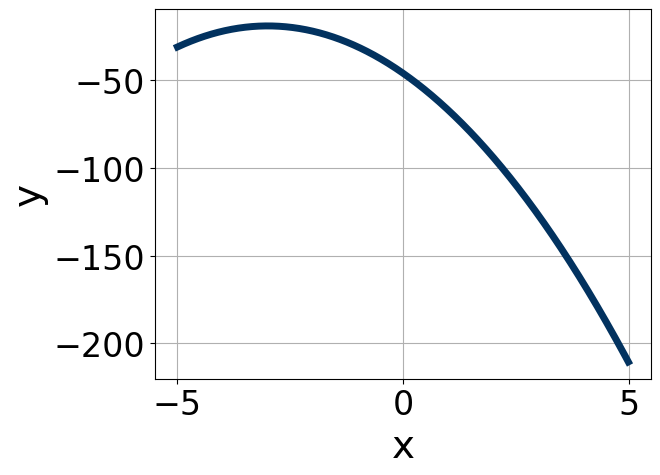
\includegraphics[width = 0.3\textwidth]{../Figures/quadraticEquationToGraphCopyAA.png}\item 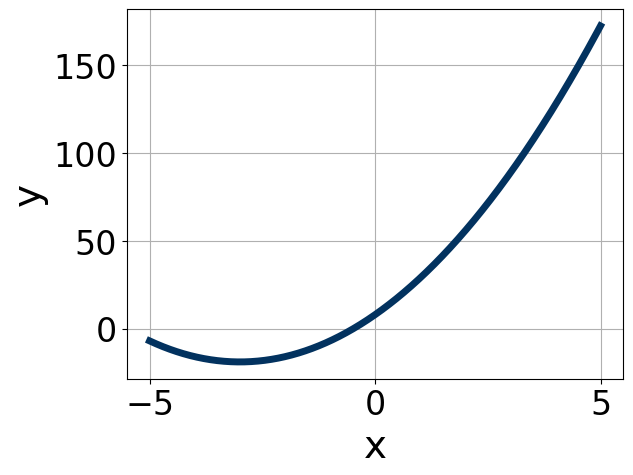
\includegraphics[width = 0.3\textwidth]{../Figures/quadraticEquationToGraphCopyBA.png}\item 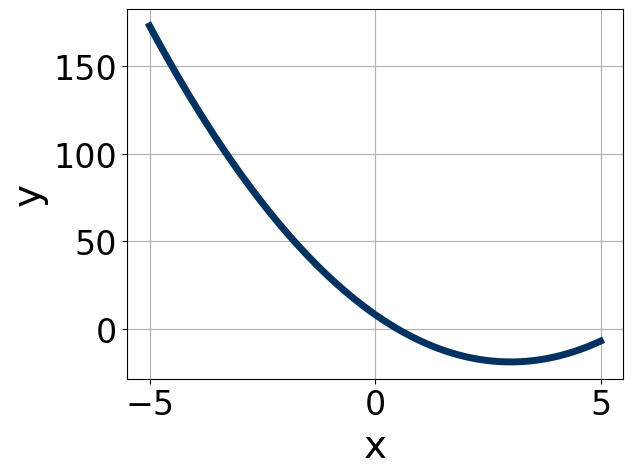
\includegraphics[width = 0.3\textwidth]{../Figures/quadraticEquationToGraphCopyCA.png}\item 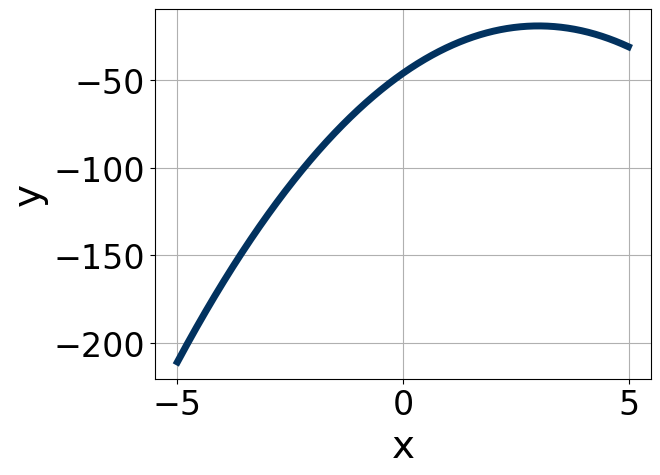
\includegraphics[width = 0.3\textwidth]{../Figures/quadraticEquationToGraphCopyDA.png}\end{multicols}\item None of the above.
\end{enumerate} }
\litem{
Solve the quadratic equation below. Then, choose the intervals that the solutions belong to, with $x_1 \leq x_2$ (if they exist).\[ 12x^{2} +7 x -9 = 0 \]\begin{enumerate}[label=\Alph*.]
\item \( x_1 \in [-1.2, -0.18] \text{ and } x_2 \in [0.9, 2.8] \)
\item \( x_1 \in [-2.69, -1.12] \text{ and } x_2 \in [-0.1, 1.2] \)
\item \( x_1 \in [-22.99, -21.32] \text{ and } x_2 \in [21, 23.8] \)
\item \( x_1 \in [-14.62, -14.4] \text{ and } x_2 \in [5.7, 8.9] \)
\item \( \text{There are no Real solutions.} \)

\end{enumerate} }
\litem{
Factor the quadratic below. Then, choose the intervals that contain the constants in the form $(ax+b)(cx+d); b \leq d.$\[ 24x^{2} +2 x -15 \]\begin{enumerate}[label=\Alph*.]
\item \( a \in [-0.18, 1.9], \hspace*{5mm} b \in [-24, -17], \hspace*{5mm} c \in [-0.9, 1.2], \text{ and } \hspace*{5mm} d \in [19, 23] \)
\item \( a \in [11.49, 13.43], \hspace*{5mm} b \in [-6, -1], \hspace*{5mm} c \in [1.4, 2.5], \text{ and } \hspace*{5mm} d \in [2, 11] \)
\item \( a \in [1.58, 2.63], \hspace*{5mm} b \in [-6, -1], \hspace*{5mm} c \in [10.2, 13.3], \text{ and } \hspace*{5mm} d \in [2, 11] \)
\item \( a \in [3.9, 5.36], \hspace*{5mm} b \in [-6, -1], \hspace*{5mm} c \in [4.6, 6.6], \text{ and } \hspace*{5mm} d \in [2, 11] \)
\item \( \text{None of the above.} \)

\end{enumerate} }
\litem{
Write the equation of the graph presented below in the form $f(x)=ax^2+bx+c$, assuming  $a=1$ or $a=-1$. Then, choose the intervals that $a, b,$ and $c$ belong to.
\begin{center}
    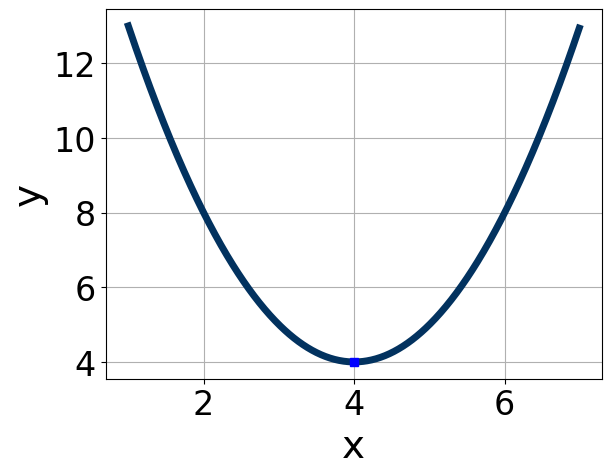
\includegraphics[width=0.5\textwidth]{../Figures/quadraticGraphToEquationB.png}
\end{center}
\begin{enumerate}[label=\Alph*.]
\item \( a \in [-2.5, -0.1], \hspace*{5mm} b \in [5, 10], \text{ and } \hspace*{5mm} c \in [-13, -8] \)
\item \( a \in [-2.5, -0.1], \hspace*{5mm} b \in [-11, -6], \text{ and } \hspace*{5mm} c \in [-13, -8] \)
\item \( a \in [-0.4, 2.4], \hspace*{5mm} b \in [-11, -6], \text{ and } \hspace*{5mm} c \in [20, 22] \)
\item \( a \in [-0.4, 2.4], \hspace*{5mm} b \in [5, 10], \text{ and } \hspace*{5mm} c \in [20, 22] \)
\item \( a \in [-0.4, 2.4], \hspace*{5mm} b \in [5, 10], \text{ and } \hspace*{5mm} c \in [11, 17] \)

\end{enumerate} }
\litem{
Solve the quadratic equation below. Then, choose the intervals that the solutions $x_1$ and $x_2$ belong to, with $x_1 \leq x_2$.\[ 25x^{2} +10 x -24 = 0 \]\begin{enumerate}[label=\Alph*.]
\item \( x_1 \in [-1.72, -0.86] \text{ and } x_2 \in [0.63, 1.34] \)
\item \( x_1 \in [-2.91, -2.08] \text{ and } x_2 \in [0.24, 0.61] \)
\item \( x_1 \in [-6.27, -5.37] \text{ and } x_2 \in [0.07, 0.26] \)
\item \( x_1 \in [-30.9, -29.8] \text{ and } x_2 \in [19.64, 20.07] \)
\item \( x_1 \in [-0.71, -0.21] \text{ and } x_2 \in [1.44, 2.11] \)

\end{enumerate} }
\litem{
Factor the quadratic below. Then, choose the intervals that contain the constants in the form $(ax+b)(cx+d); b \leq d.$\[ 16x^{2} -8 x -15 \]\begin{enumerate}[label=\Alph*.]
\item \( a \in [3.09, 4.32], \hspace*{5mm} b \in [-7, 2], \hspace*{5mm} c \in [3.36, 4.31], \text{ and } \hspace*{5mm} d \in [-3, 8] \)
\item \( a \in [7.27, 8.73], \hspace*{5mm} b \in [-7, 2], \hspace*{5mm} c \in [1.7, 2.33], \text{ and } \hspace*{5mm} d \in [-3, 8] \)
\item \( a \in [0.89, 1.59], \hspace*{5mm} b \in [-26, -15], \hspace*{5mm} c \in [0.43, 1.16], \text{ and } \hspace*{5mm} d \in [10, 15] \)
\item \( a \in [1.85, 2.78], \hspace*{5mm} b \in [-7, 2], \hspace*{5mm} c \in [7.25, 8.92], \text{ and } \hspace*{5mm} d \in [-3, 8] \)
\item \( \text{None of the above.} \)

\end{enumerate} }
\litem{
Write the equation of the graph presented below in the form $f(x)=ax^2+bx+c$, assuming  $a=1$ or $a=-1$. Then, choose the intervals that $a, b,$ and $c$ belong to.
\begin{center}
    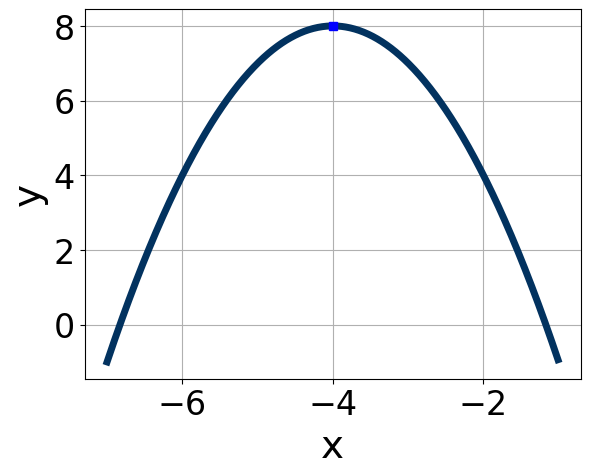
\includegraphics[width=0.5\textwidth]{../Figures/quadraticGraphToEquationCopyB.png}
\end{center}
\begin{enumerate}[label=\Alph*.]
\item \( a \in [-3, 0], \hspace*{5mm} b \in [8, 12], \text{ and } \hspace*{5mm} c \in [-9, -4] \)
\item \( a \in [-3, 0], \hspace*{5mm} b \in [-11, -6], \text{ and } \hspace*{5mm} c \in [-9, -4] \)
\item \( a \in [-3, 0], \hspace*{5mm} b \in [8, 12], \text{ and } \hspace*{5mm} c \in [-26, -22] \)
\item \( a \in [1, 4], \hspace*{5mm} b \in [-11, -6], \text{ and } \hspace*{5mm} c \in [22, 27] \)
\item \( a \in [1, 4], \hspace*{5mm} b \in [8, 12], \text{ and } \hspace*{5mm} c \in [22, 27] \)

\end{enumerate} }
\litem{
Graph the equation below.\[ f(x) = (x-2)^2 + 11 \]\begin{enumerate}[label=\Alph*.]
\begin{multicols}{2}\item 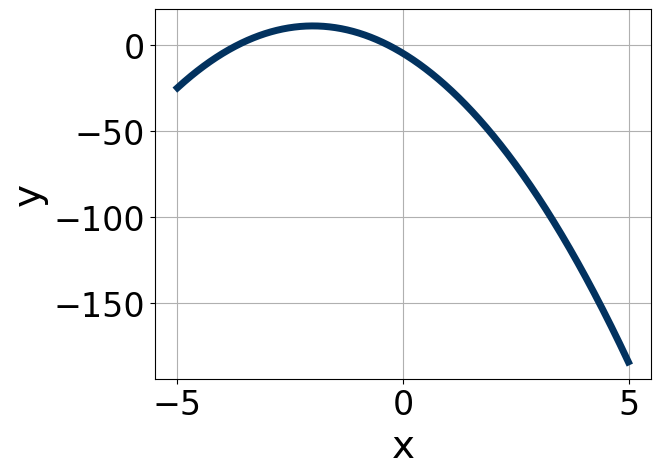
\includegraphics[width = 0.3\textwidth]{../Figures/quadraticEquationToGraphAB.png}\item 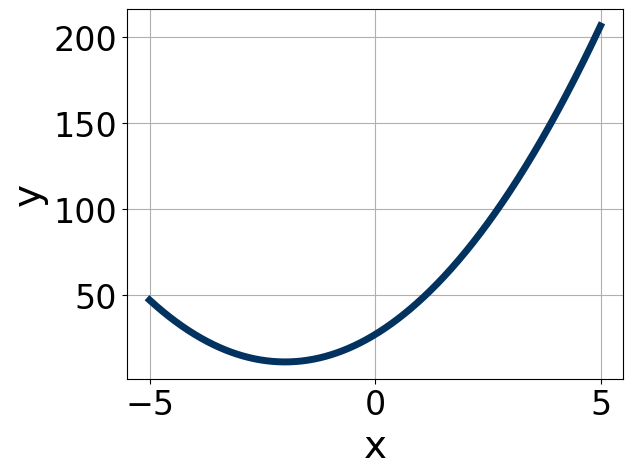
\includegraphics[width = 0.3\textwidth]{../Figures/quadraticEquationToGraphBB.png}\item 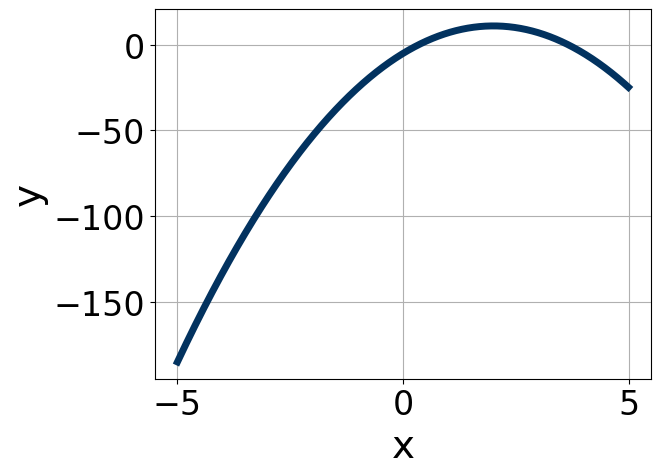
\includegraphics[width = 0.3\textwidth]{../Figures/quadraticEquationToGraphCB.png}\item 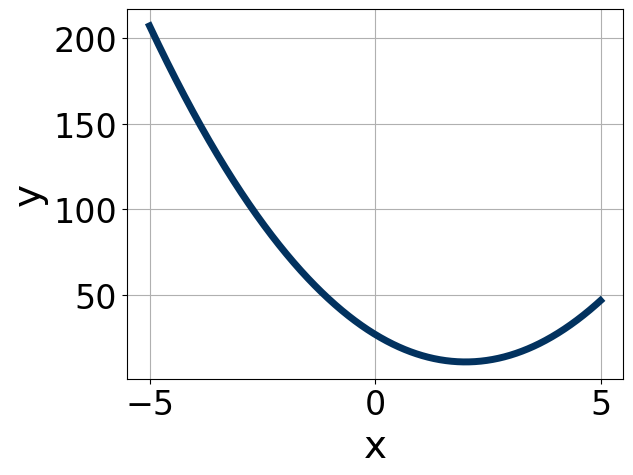
\includegraphics[width = 0.3\textwidth]{../Figures/quadraticEquationToGraphDB.png}\end{multicols}\item None of the above.
\end{enumerate} }
\litem{
Solve the quadratic equation below. Then, choose the intervals that the solutions belong to, with $x_1 \leq x_2$ (if they exist).\[ -10x^{2} -15 x + 2 = 0 \]\begin{enumerate}[label=\Alph*.]
\item \( x_1 \in [-19.3, -16.5] \text{ and } x_2 \in [16.6, 17.1] \)
\item \( x_1 \in [-0.5, 1.1] \text{ and } x_2 \in [1.3, 2.2] \)
\item \( x_1 \in [-3.6, -1.4] \text{ and } x_2 \in [-0.6, 0.6] \)
\item \( x_1 \in [-1.6, -0.9] \text{ and } x_2 \in [16.2, 16.5] \)
\item \( \text{There are no Real solutions.} \)

\end{enumerate} }
\litem{
Solve the quadratic equation below. Then, choose the intervals that the solutions $x_1$ and $x_2$ belong to, with $x_1 \leq x_2$.\[ 25x^{2} +60 x + 36 = 0 \]\begin{enumerate}[label=\Alph*.]
\item \( x_1 \in [-3.4, -1.82] \text{ and } x_2 \in [-0.68, -0.56] \)
\item \( x_1 \in [-4.42, -3.57] \text{ and } x_2 \in [-0.58, -0.25] \)
\item \( x_1 \in [-1.43, -0.68] \text{ and } x_2 \in [-1.26, -1.18] \)
\item \( x_1 \in [-6.71, -4.51] \text{ and } x_2 \in [-0.35, -0.02] \)
\item \( x_1 \in [-30.83, -29.51] \text{ and } x_2 \in [-30.04, -29.95] \)

\end{enumerate} }
\litem{
Graph the equation below.\[ f(x) = -(x-3)^2 - 18 \]\begin{enumerate}[label=\Alph*.]
\begin{multicols}{2}\item 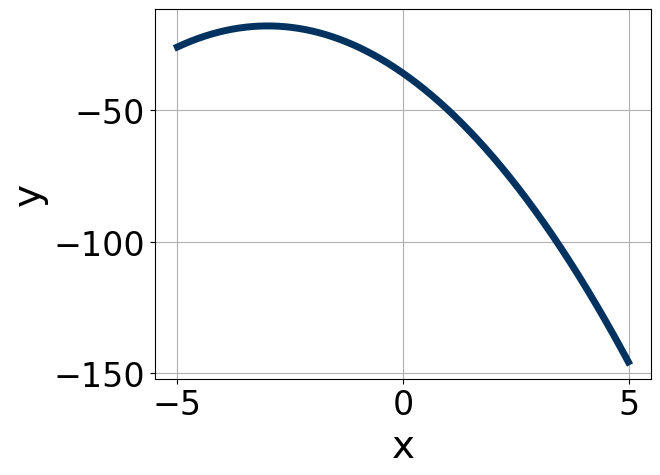
\includegraphics[width = 0.3\textwidth]{../Figures/quadraticEquationToGraphCopyAB.png}\item 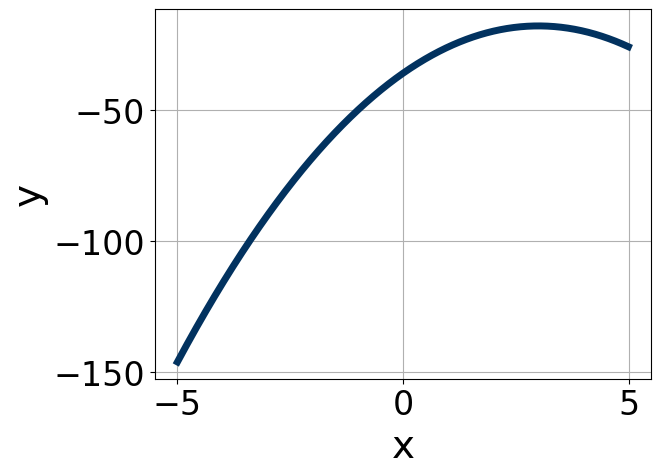
\includegraphics[width = 0.3\textwidth]{../Figures/quadraticEquationToGraphCopyBB.png}\item 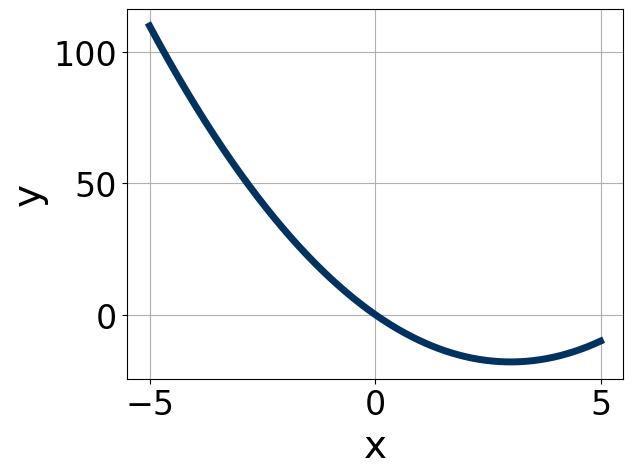
\includegraphics[width = 0.3\textwidth]{../Figures/quadraticEquationToGraphCopyCB.png}\item 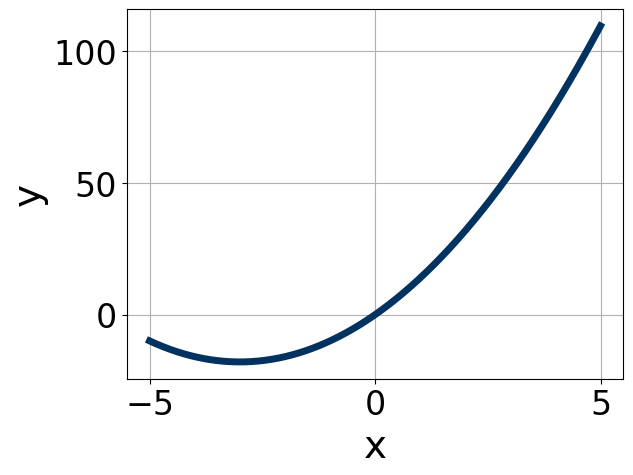
\includegraphics[width = 0.3\textwidth]{../Figures/quadraticEquationToGraphCopyDB.png}\end{multicols}\item None of the above.
\end{enumerate} }
\litem{
Solve the quadratic equation below. Then, choose the intervals that the solutions belong to, with $x_1 \leq x_2$ (if they exist).\[ 18x^{2} -14 x -6 = 0 \]\begin{enumerate}[label=\Alph*.]
\item \( x_1 \in [-25.9, -23.6] \text{ and } x_2 \in [24.99, 25.75] \)
\item \( x_1 \in [-6.8, -4.8] \text{ and } x_2 \in [18.51, 19.73] \)
\item \( x_1 \in [-2.6, -0.4] \text{ and } x_2 \in [-0.51, 0.31] \)
\item \( x_1 \in [-0.6, -0.2] \text{ and } x_2 \in [0.98, 1.55] \)
\item \( \text{There are no Real solutions.} \)

\end{enumerate} }
\litem{
Factor the quadratic below. Then, choose the intervals that contain the constants in the form $(ax+b)(cx+d); b \leq d.$\[ 36x^{2} +7 x -15 \]\begin{enumerate}[label=\Alph*.]
\item \( a \in [1.2, 4.7], \hspace*{5mm} b \in [-11, 5], \hspace*{5mm} c \in [6.3, 8.6], \text{ and } \hspace*{5mm} d \in [2, 5] \)
\item \( a \in [6.8, 9.5], \hspace*{5mm} b \in [-11, 5], \hspace*{5mm} c \in [1.8, 4.8], \text{ and } \hspace*{5mm} d \in [2, 5] \)
\item \( a \in [26.6, 27.8], \hspace*{5mm} b \in [-11, 5], \hspace*{5mm} c \in [-0.9, 1.5], \text{ and } \hspace*{5mm} d \in [2, 5] \)
\item \( a \in [-0.1, 2.7], \hspace*{5mm} b \in [-24, -16], \hspace*{5mm} c \in [-0.9, 1.5], \text{ and } \hspace*{5mm} d \in [27, 30] \)
\item \( \text{None of the above.} \)

\end{enumerate} }
\litem{
Write the equation of the graph presented below in the form $f(x)=ax^2+bx+c$, assuming  $a=1$ or $a=-1$. Then, choose the intervals that $a, b,$ and $c$ belong to.
\begin{center}
    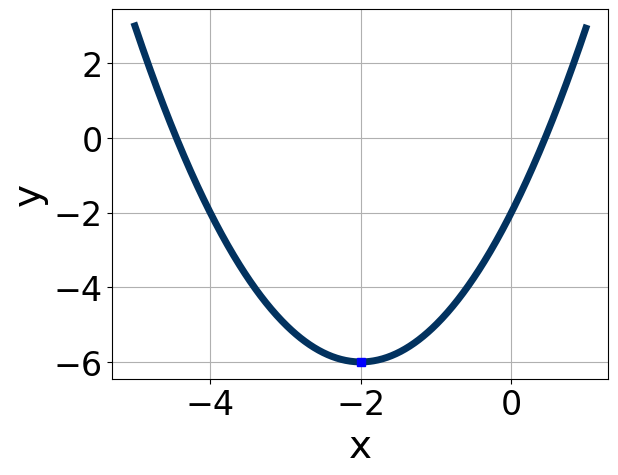
\includegraphics[width=0.5\textwidth]{../Figures/quadraticGraphToEquationC.png}
\end{center}
\begin{enumerate}[label=\Alph*.]
\item \( a \in [0.9, 1.7], \hspace*{5mm} b \in [-5, 1], \text{ and } \hspace*{5mm} c \in [-3, 2] \)
\item \( a \in [-1.1, -0.7], \hspace*{5mm} b \in [-5, 1], \text{ and } \hspace*{5mm} c \in [-12, -9] \)
\item \( a \in [0.9, 1.7], \hspace*{5mm} b \in [-5, 1], \text{ and } \hspace*{5mm} c \in [10, 11] \)
\item \( a \in [-1.1, -0.7], \hspace*{5mm} b \in [1, 6], \text{ and } \hspace*{5mm} c \in [-12, -9] \)
\item \( a \in [0.9, 1.7], \hspace*{5mm} b \in [1, 6], \text{ and } \hspace*{5mm} c \in [-3, 2] \)

\end{enumerate} }
\litem{
Solve the quadratic equation below. Then, choose the intervals that the solutions $x_1$ and $x_2$ belong to, with $x_1 \leq x_2$.\[ 25x^{2} -60 x + 36 = 0 \]\begin{enumerate}[label=\Alph*.]
\item \( x_1 \in [29.89, 30.07] \text{ and } x_2 \in [28.82, 30.39] \)
\item \( x_1 \in [0.29, 0.4] \text{ and } x_2 \in [2.8, 5.36] \)
\item \( x_1 \in [0.98, 1.27] \text{ and } x_2 \in [0.98, 1.24] \)
\item \( x_1 \in [0.5, 0.69] \text{ and } x_2 \in [2, 2.82] \)
\item \( x_1 \in [0.18, 0.24] \text{ and } x_2 \in [5.82, 8.14] \)

\end{enumerate} }
\litem{
Factor the quadratic below. Then, choose the intervals that contain the constants in the form $(ax+b)(cx+d); b \leq d.$\[ 54x^{2} -57 x + 10 \]\begin{enumerate}[label=\Alph*.]
\item \( a \in [0.39, 1.72], \hspace*{5mm} b \in [-45, -42], \hspace*{5mm} c \in [0.4, 2.2], \text{ and } \hspace*{5mm} d \in [-14, -6] \)
\item \( a \in [1.62, 2.98], \hspace*{5mm} b \in [-7, -1], \hspace*{5mm} c \in [26.1, 27.8], \text{ and } \hspace*{5mm} d \in [-3, 0] \)
\item \( a \in [5.69, 6.25], \hspace*{5mm} b \in [-7, -1], \hspace*{5mm} c \in [7.2, 9.6], \text{ and } \hspace*{5mm} d \in [-3, 0] \)
\item \( a \in [11.54, 12.85], \hspace*{5mm} b \in [-7, -1], \hspace*{5mm} c \in [3.6, 6.5], \text{ and } \hspace*{5mm} d \in [-3, 0] \)
\item \( \text{None of the above.} \)

\end{enumerate} }
\litem{
Write the equation of the graph presented below in the form $f(x)=ax^2+bx+c$, assuming  $a=1$ or $a=-1$. Then, choose the intervals that $a, b,$ and $c$ belong to.
\begin{center}
    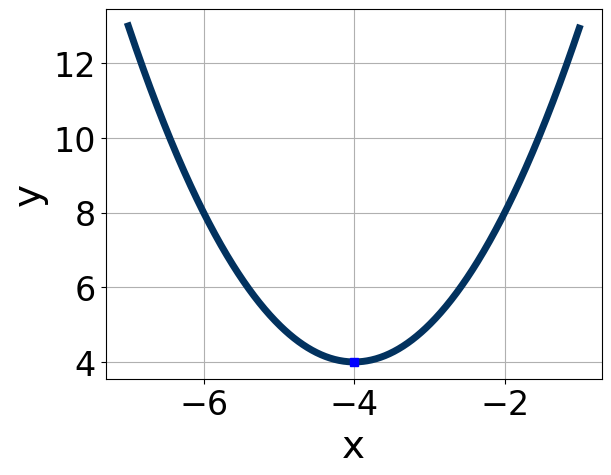
\includegraphics[width=0.5\textwidth]{../Figures/quadraticGraphToEquationCopyC.png}
\end{center}
\begin{enumerate}[label=\Alph*.]
\item \( a \in [-1.8, 0.9], \hspace*{5mm} b \in [-9, -4], \text{ and } \hspace*{5mm} c \in [-15, -11] \)
\item \( a \in [-0.6, 1.1], \hspace*{5mm} b \in [-9, -4], \text{ and } \hspace*{5mm} c \in [17, 22] \)
\item \( a \in [-0.6, 1.1], \hspace*{5mm} b \in [7, 13], \text{ and } \hspace*{5mm} c \in [17, 22] \)
\item \( a \in [-1.8, 0.9], \hspace*{5mm} b \in [7, 13], \text{ and } \hspace*{5mm} c \in [-15, -11] \)
\item \( a \in [-0.6, 1.1], \hspace*{5mm} b \in [-9, -4], \text{ and } \hspace*{5mm} c \in [12, 13] \)

\end{enumerate} }
\litem{
Graph the equation below.\[ f(x) = -(x+2)^2 + 10 \]\begin{enumerate}[label=\Alph*.]
\begin{multicols}{2}\item 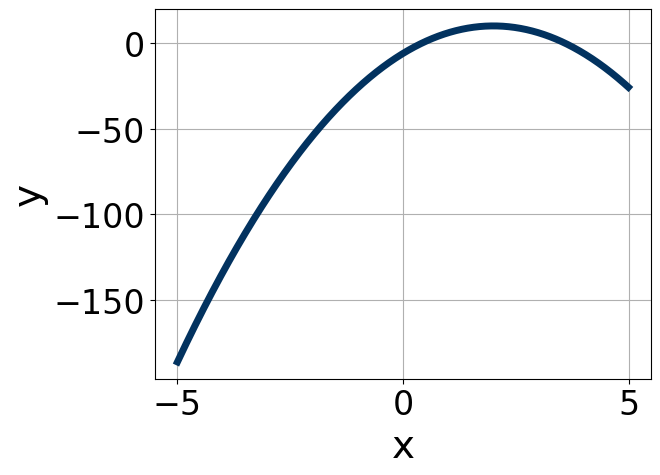
\includegraphics[width = 0.3\textwidth]{../Figures/quadraticEquationToGraphAC.png}\item 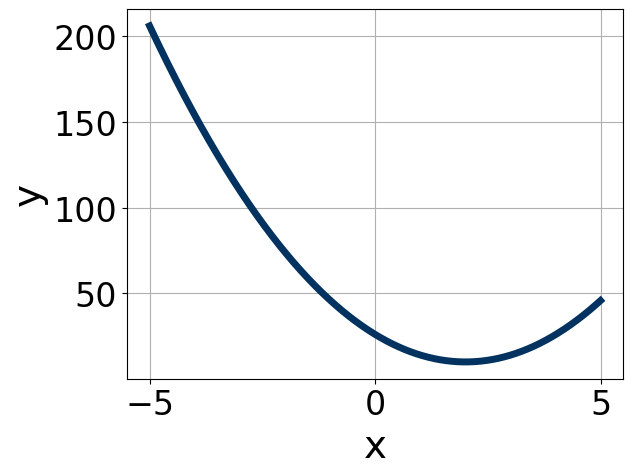
\includegraphics[width = 0.3\textwidth]{../Figures/quadraticEquationToGraphBC.png}\item 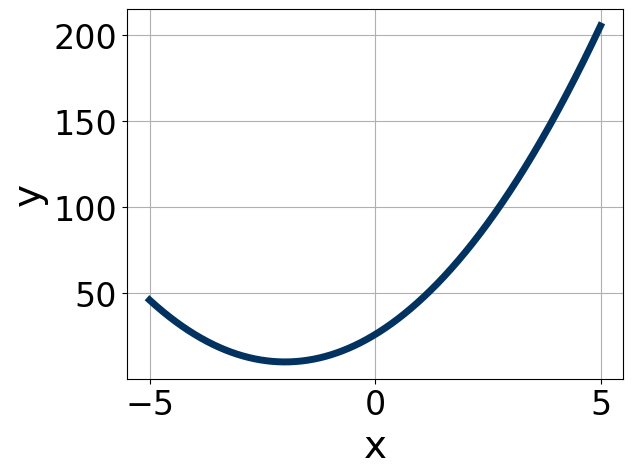
\includegraphics[width = 0.3\textwidth]{../Figures/quadraticEquationToGraphCC.png}\item 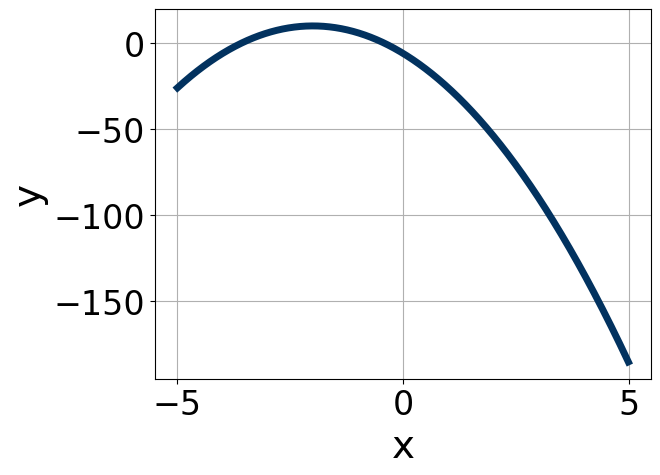
\includegraphics[width = 0.3\textwidth]{../Figures/quadraticEquationToGraphDC.png}\end{multicols}\item None of the above.
\end{enumerate} }
\litem{
Solve the quadratic equation below. Then, choose the intervals that the solutions belong to, with $x_1 \leq x_2$ (if they exist).\[ 18x^{2} +10 x -7 = 0 \]\begin{enumerate}[label=\Alph*.]
\item \( x_1 \in [-25.15, -23.62] \text{ and } x_2 \in [23.8, 26] \)
\item \( x_1 \in [-0.79, 0.13] \text{ and } x_2 \in [0.9, 1.5] \)
\item \( x_1 \in [-17.42, -17.07] \text{ and } x_2 \in [6.4, 8.4] \)
\item \( x_1 \in [-0.99, -0.95] \text{ and } x_2 \in [-0.2, 0.9] \)
\item \( \text{There are no Real solutions.} \)

\end{enumerate} }
\litem{
Solve the quadratic equation below. Then, choose the intervals that the solutions $x_1$ and $x_2$ belong to, with $x_1 \leq x_2$.\[ 20x^{2} -21 x -54 = 0 \]\begin{enumerate}[label=\Alph*.]
\item \( x_1 \in [-3.95, -3.57] \text{ and } x_2 \in [0.52, 2.17] \)
\item \( x_1 \in [-24.11, -23.57] \text{ and } x_2 \in [44.9, 46.39] \)
\item \( x_1 \in [-6.19, -5.88] \text{ and } x_2 \in [-0.33, 0.48] \)
\item \( x_1 \in [-1.76, -1.17] \text{ and } x_2 \in [2.03, 2.41] \)
\item \( x_1 \in [-0.8, 0.32] \text{ and } x_2 \in [5.83, 7.15] \)

\end{enumerate} }
\litem{
Graph the equation below.\[ f(x) = -(x-1)^2 - 13 \]\begin{enumerate}[label=\Alph*.]
\begin{multicols}{2}\item 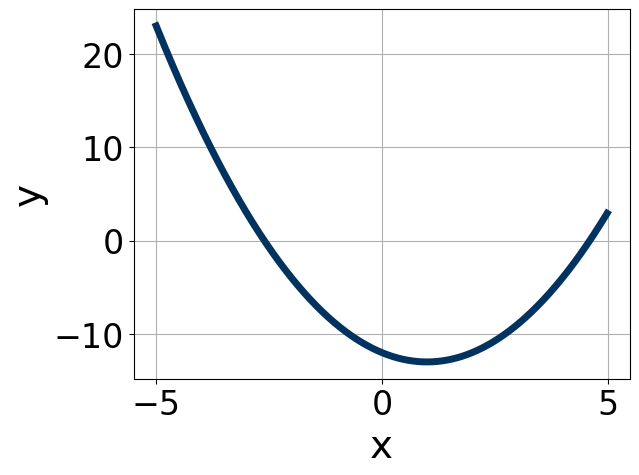
\includegraphics[width = 0.3\textwidth]{../Figures/quadraticEquationToGraphCopyAC.png}\item 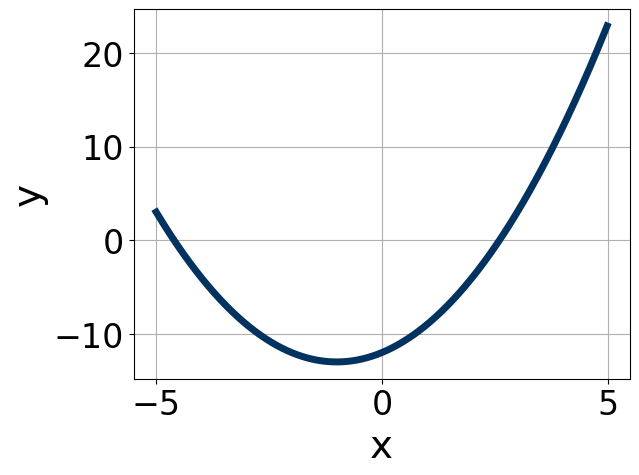
\includegraphics[width = 0.3\textwidth]{../Figures/quadraticEquationToGraphCopyBC.png}\item 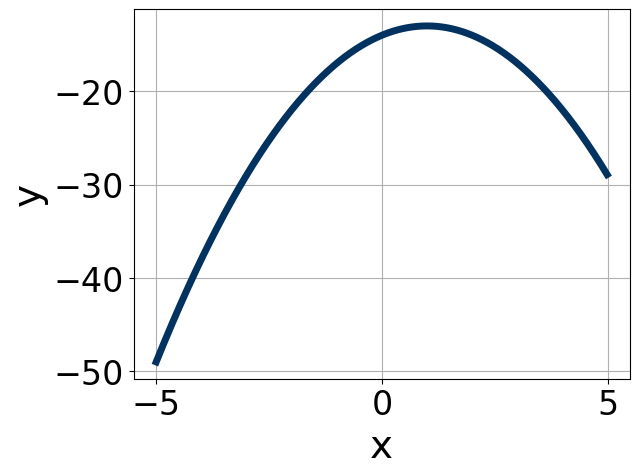
\includegraphics[width = 0.3\textwidth]{../Figures/quadraticEquationToGraphCopyCC.png}\item 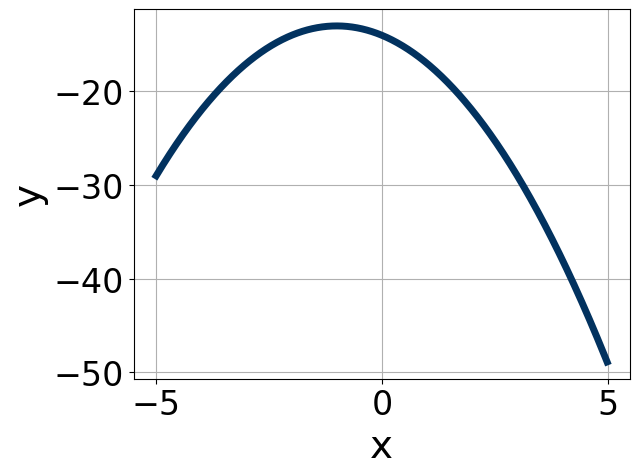
\includegraphics[width = 0.3\textwidth]{../Figures/quadraticEquationToGraphCopyDC.png}\end{multicols}\item None of the above.
\end{enumerate} }
\litem{
Solve the quadratic equation below. Then, choose the intervals that the solutions belong to, with $x_1 \leq x_2$ (if they exist).\[ 12x^{2} +12 x -7 = 0 \]\begin{enumerate}[label=\Alph*.]
\item \( x_1 \in [-0.86, 0.31] \text{ and } x_2 \in [0.8, 2.3] \)
\item \( x_1 \in [-22.76, -21.95] \text{ and } x_2 \in [21.3, 22.1] \)
\item \( x_1 \in [-1.58, -0.97] \text{ and } x_2 \in [-1.3, 0.9] \)
\item \( x_1 \in [-17.73, -16.66] \text{ and } x_2 \in [3.1, 6.8] \)
\item \( \text{There are no Real solutions.} \)

\end{enumerate} }
\litem{
Factor the quadratic below. Then, choose the intervals that contain the constants in the form $(ax+b)(cx+d); b \leq d.$\[ 36x^{2} -60 x + 25 \]\begin{enumerate}[label=\Alph*.]
\item \( a \in [-2.3, 2.1], \hspace*{5mm} b \in [-31, -29], \hspace*{5mm} c \in [0.8, 1.8], \text{ and } \hspace*{5mm} d \in [-34, -25] \)
\item \( a \in [2.9, 4], \hspace*{5mm} b \in [-5, -2], \hspace*{5mm} c \in [11.6, 13.9], \text{ and } \hspace*{5mm} d \in [-6, -2] \)
\item \( a \in [4.9, 6.6], \hspace*{5mm} b \in [-5, -2], \hspace*{5mm} c \in [3.4, 6.6], \text{ and } \hspace*{5mm} d \in [-6, -2] \)
\item \( a \in [16.9, 18.3], \hspace*{5mm} b \in [-5, -2], \hspace*{5mm} c \in [1.5, 3.2], \text{ and } \hspace*{5mm} d \in [-6, -2] \)
\item \( \text{None of the above.} \)

\end{enumerate} }
\end{enumerate}

\end{document}